\chapter{Additional Results}
\label{att:add_results}

\section{SBS Comparisons}

Small collection of side by side comparisons between the models.
\begin{figure}[H]
  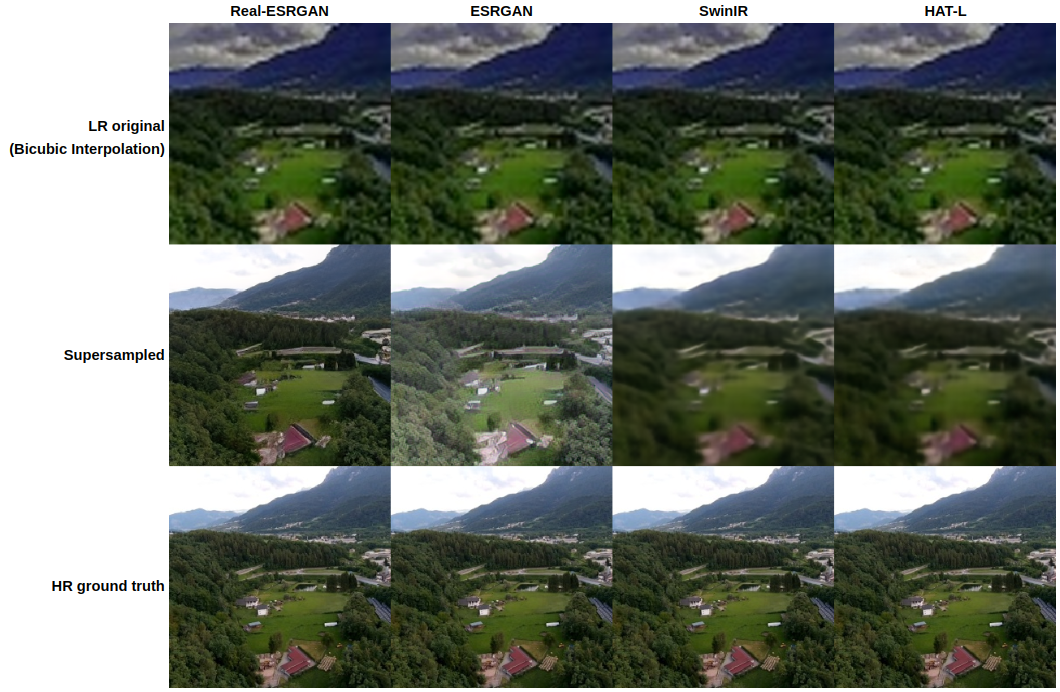
\includegraphics[width=1\textwidth]{figures/allegati/sbs_1.png}
  \label{img:sbs1}
\end{figure}
\begin{figure}[H]
  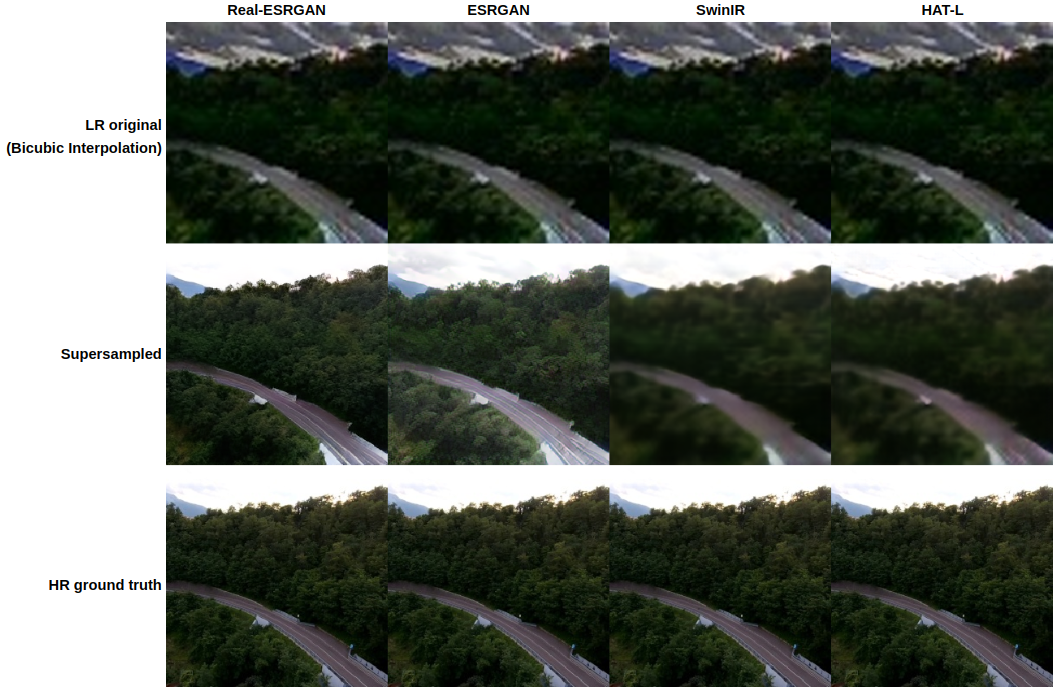
\includegraphics[width=1\textwidth]{figures/allegati/sbs_2.png}
  \label{img:sbs2}
\end{figure}
\begin{figure}[H]
  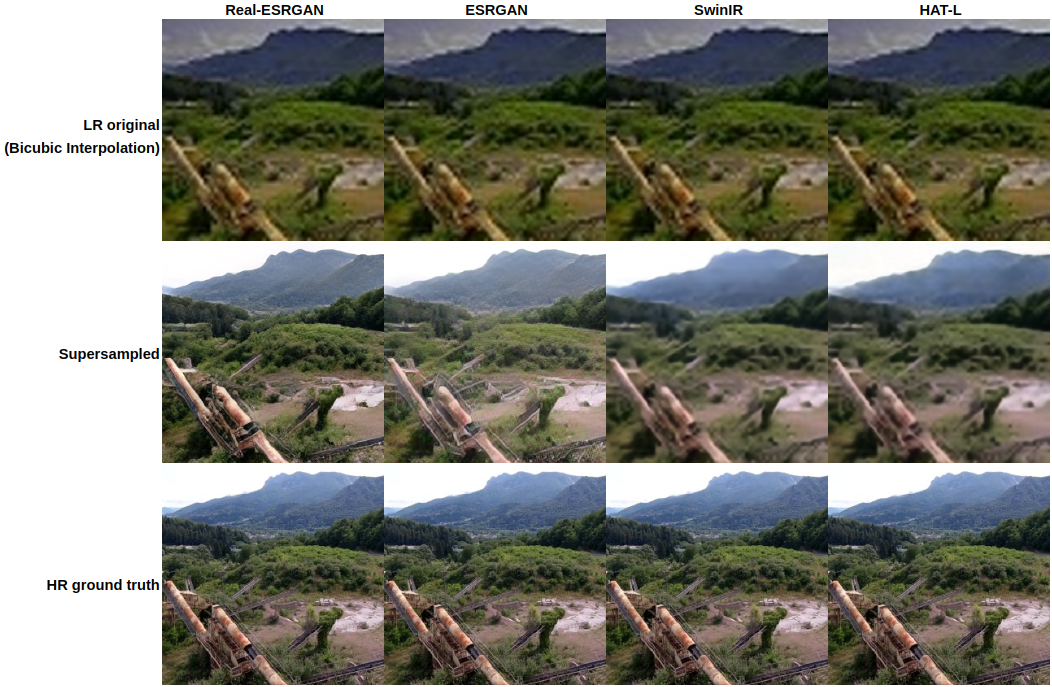
\includegraphics[width=1\textwidth]{figures/allegati/sbs_3.png}
  \label{img:sbs3}
\end{figure}

\newpage
\section{Supersampled Images}
All the images are, from top to bottom, orignal LR resized to 4 times its orignal size with bicubic interpolation, generated image by supersampling with scale 4, HR ground truth.

\subsection{ESRGAN}

\begin{figure}[H]
  \centering
  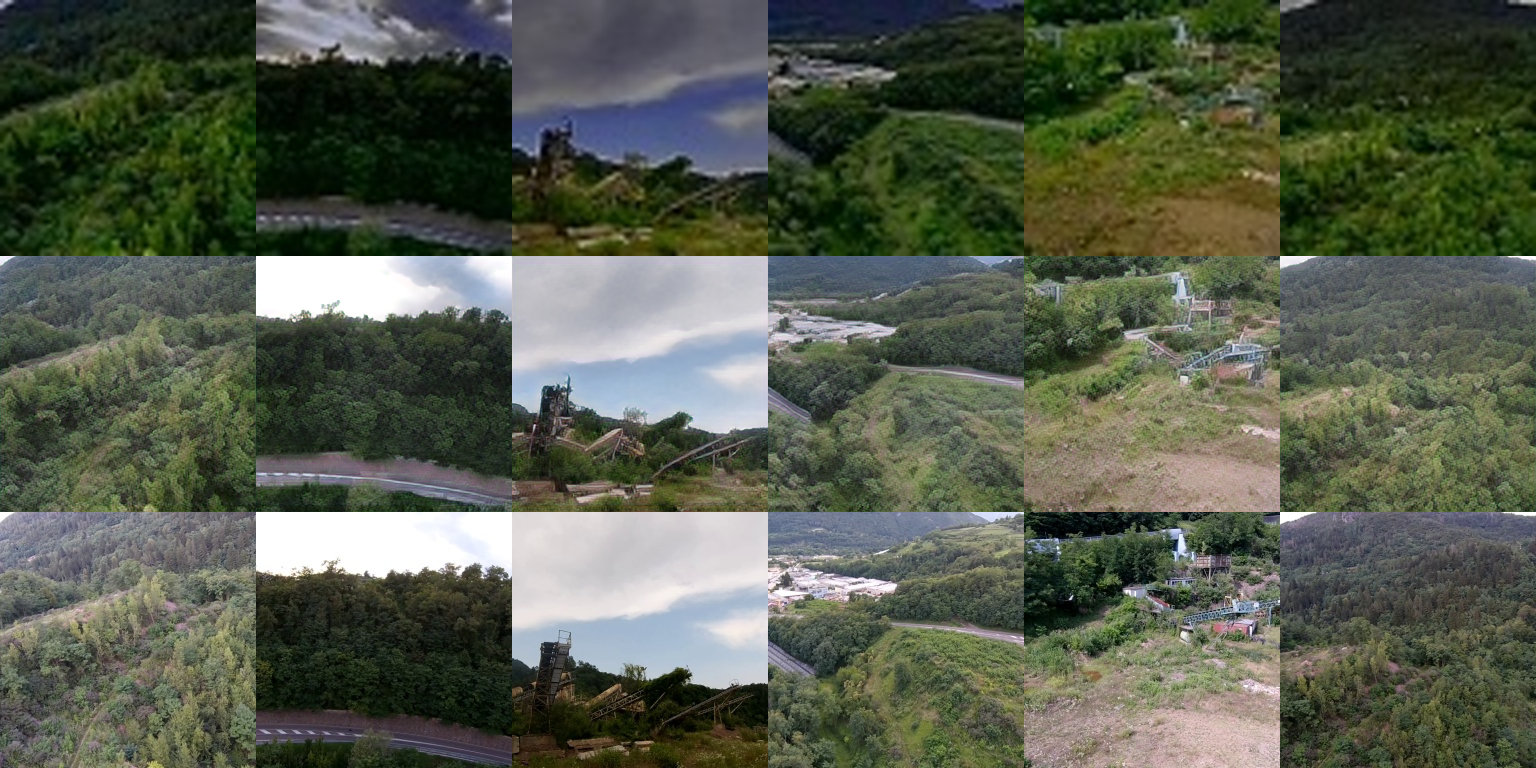
\includegraphics[width=1\textwidth]{figures/allegati/esrgan_64.png}
  \caption{From the 64 to 256 dataset.}
  \label{img:esrgan_att}
\end{figure}

\begin{figure}[H]
  \centering
  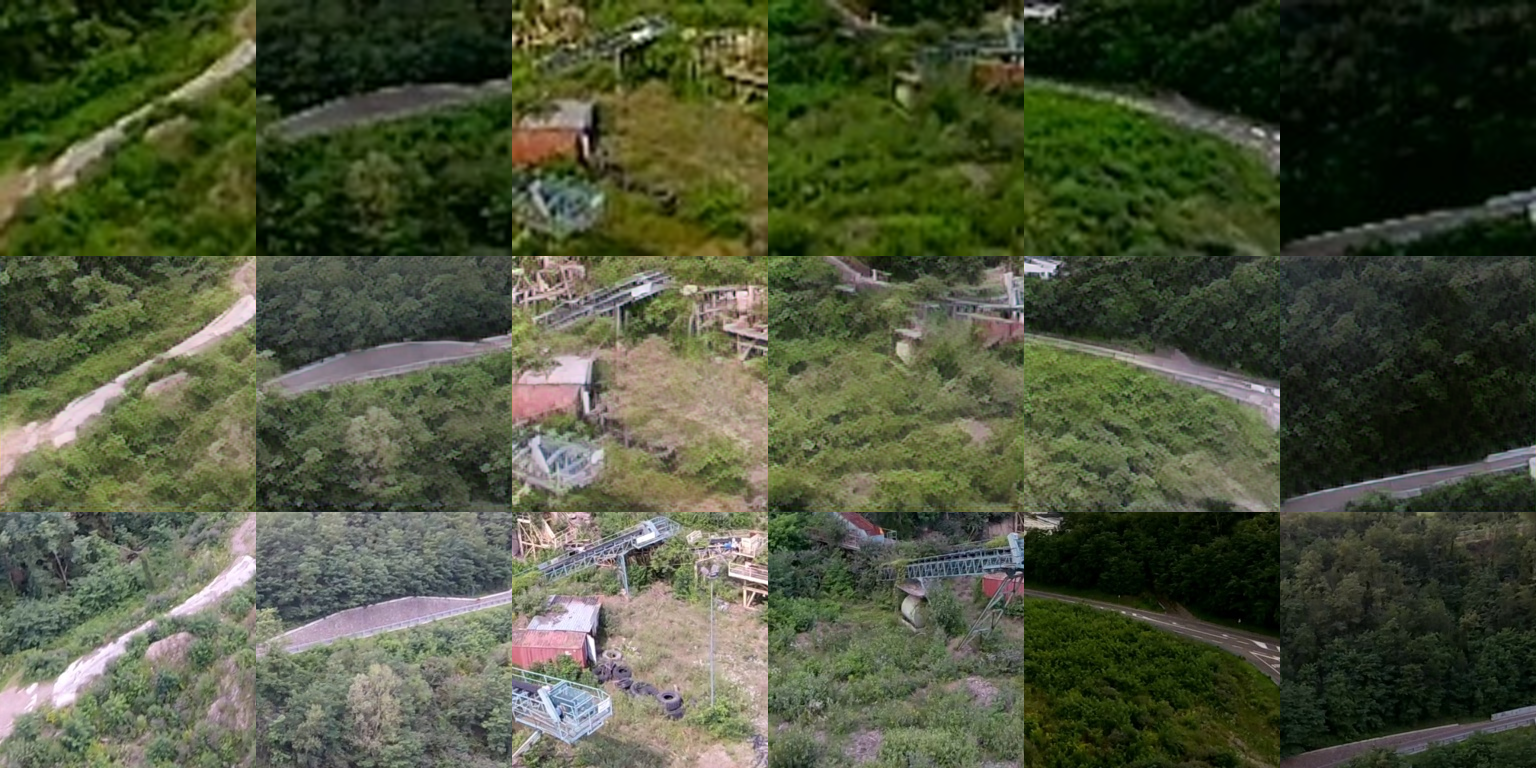
\includegraphics[width=1\textwidth]{figures/allegati/esrgan_64_patches.png}
  \caption{From the 64 to 256 patches dataset.}
  \label{img:esrgan_att}
\end{figure}

\begin{figure}[H]
  \centering
  \includegraphics[width=1\textwidth]{figures/allegati/esrgan_128.png}
  \caption{From the 128 to 512 dataset.}
  \label{img:esrgan_att}
\end{figure}

\subsection{Real-ESRGAN}

\begin{figure}[H]
  \centering
  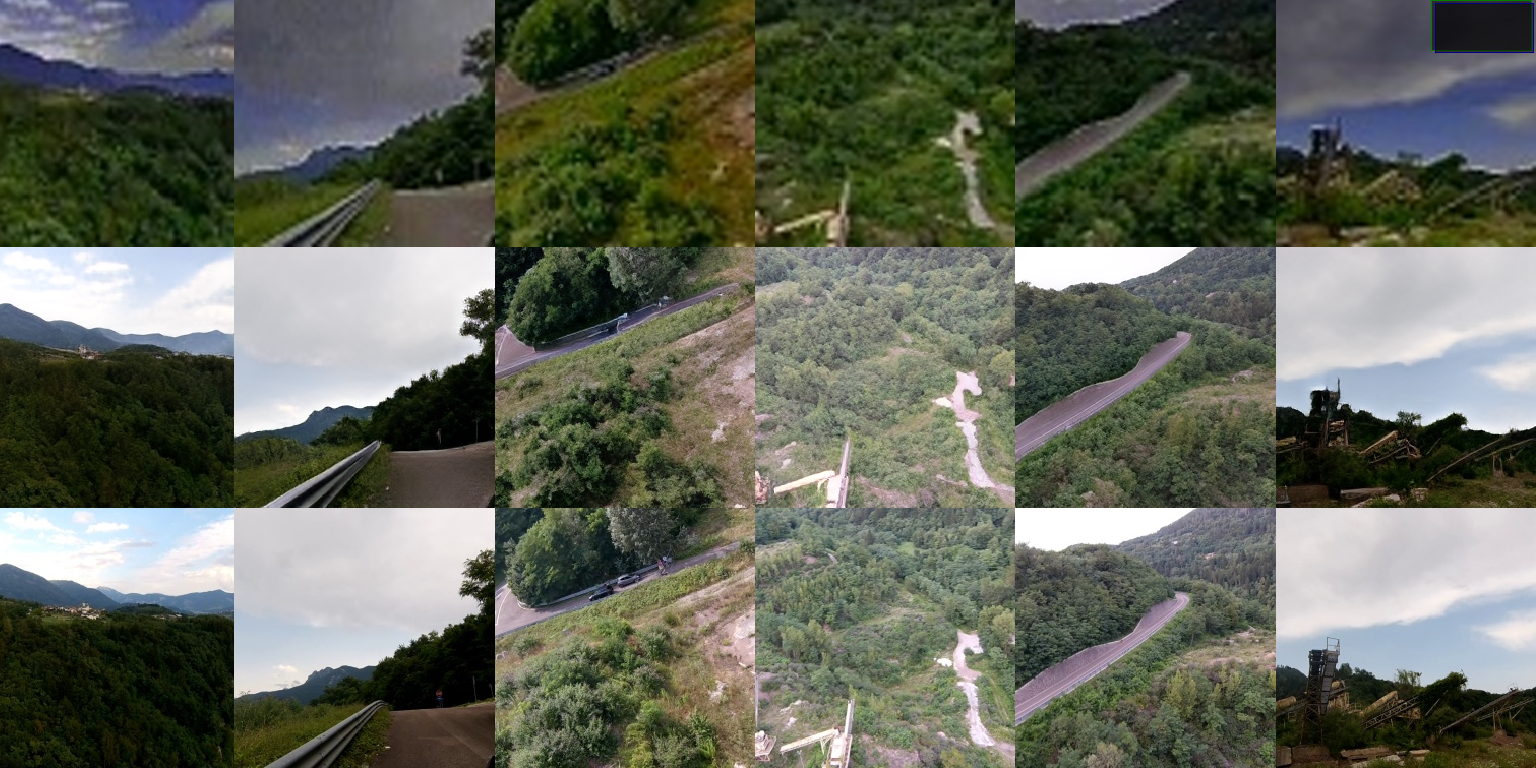
\includegraphics[width=1\textwidth]{figures/allegati/realesrgan_64_3.png}
  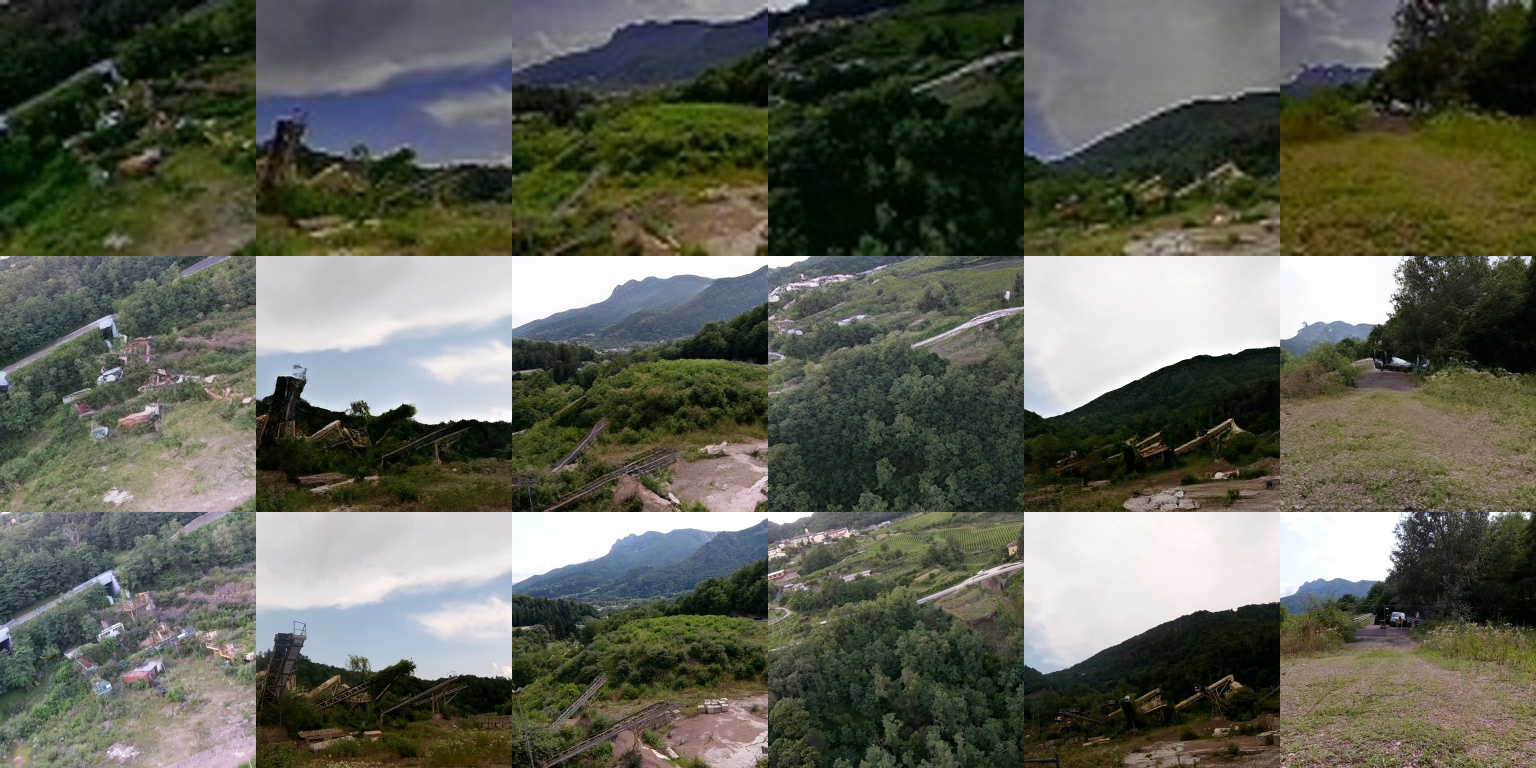
\includegraphics[width=1\textwidth]{figures/allegati/realesrgan_64_4.png}
  \caption{From the 64 to 256 dataset.}
  \label{img:realesrgan_att}
\end{figure}

\begin{figure}[H]
  \centering
  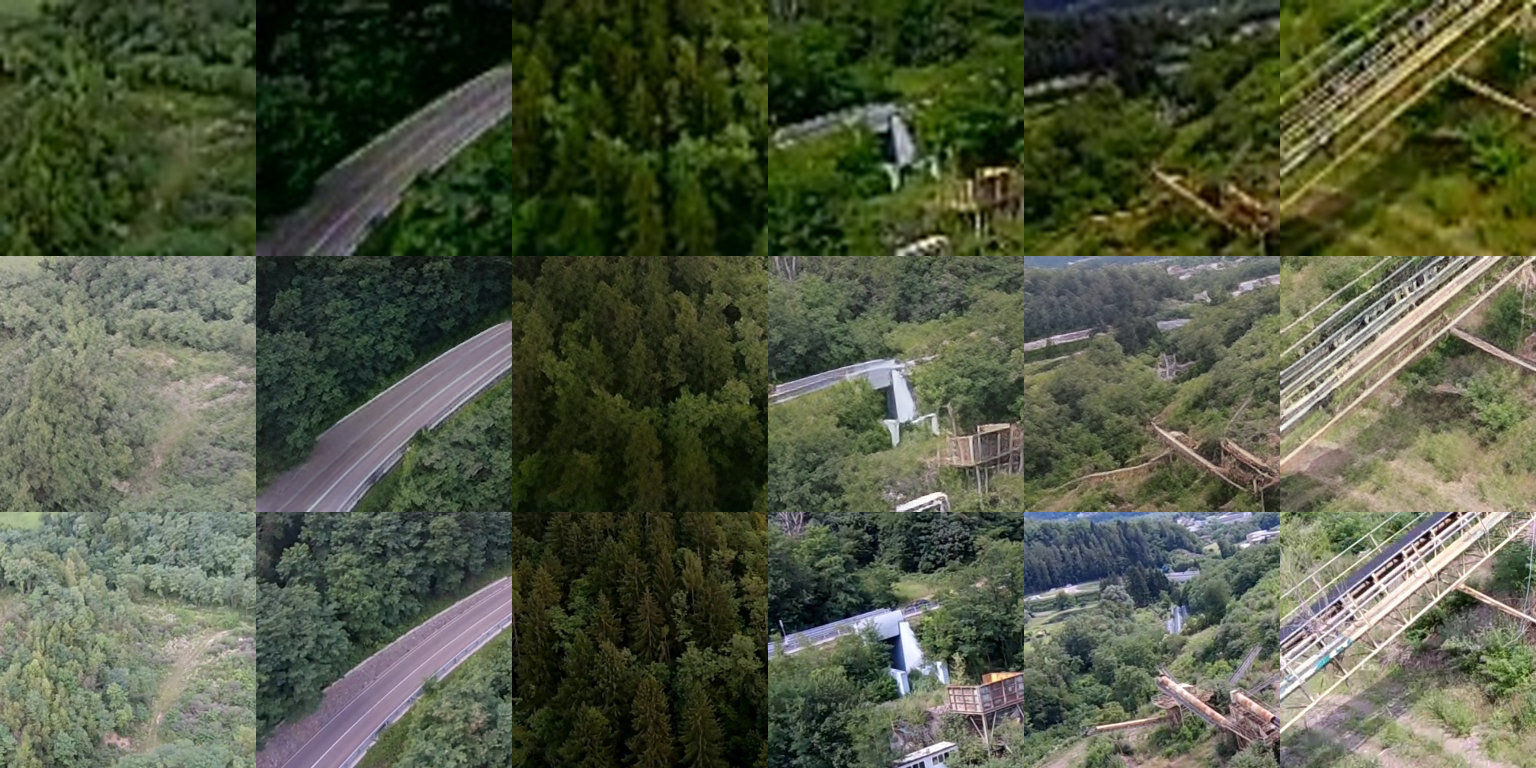
\includegraphics[width=1\textwidth]{figures/allegati/realesrgan_64_patches.png}
  \caption{From the 64 to 256 patches dataset.}
  \label{img:realesrgan_att}
\end{figure}

\begin{figure}[H]
  \centering
  \includegraphics[width=1\textwidth]{figures/allegati/realesrgan_128.png}
  \caption{From the 128 to 512 dataset.}
  \label{img:realesrgan_att}
\end{figure}

\subsection{SwinIR}

\begin{figure}[H]
  \centering
  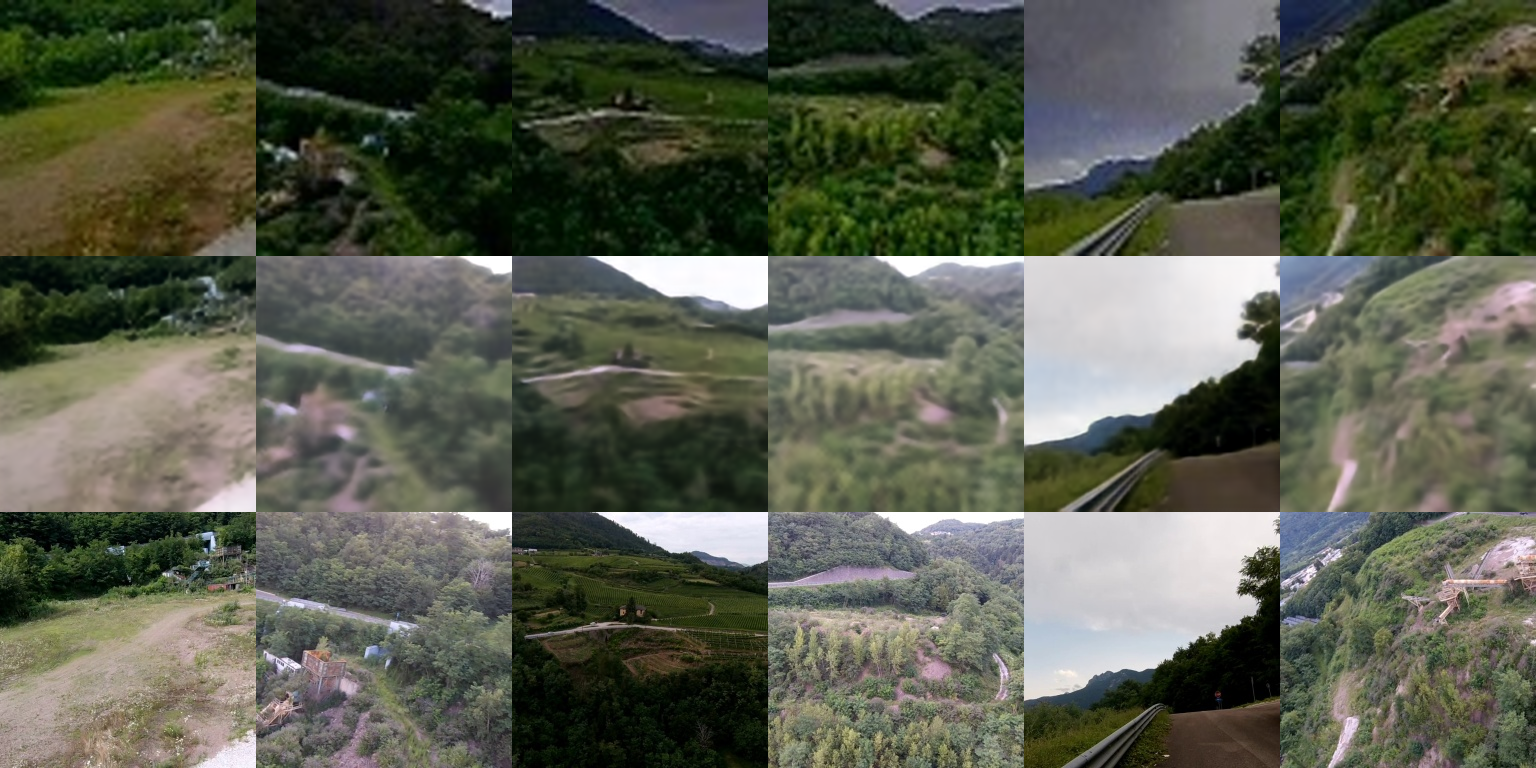
\includegraphics[width=1\textwidth]{figures/allegati/swinir_64.png}
  \caption{From the 64 to 256 dataset.}
  \label{img:esrgan_att}
\end{figure}

\begin{figure}[H]
  \centering
  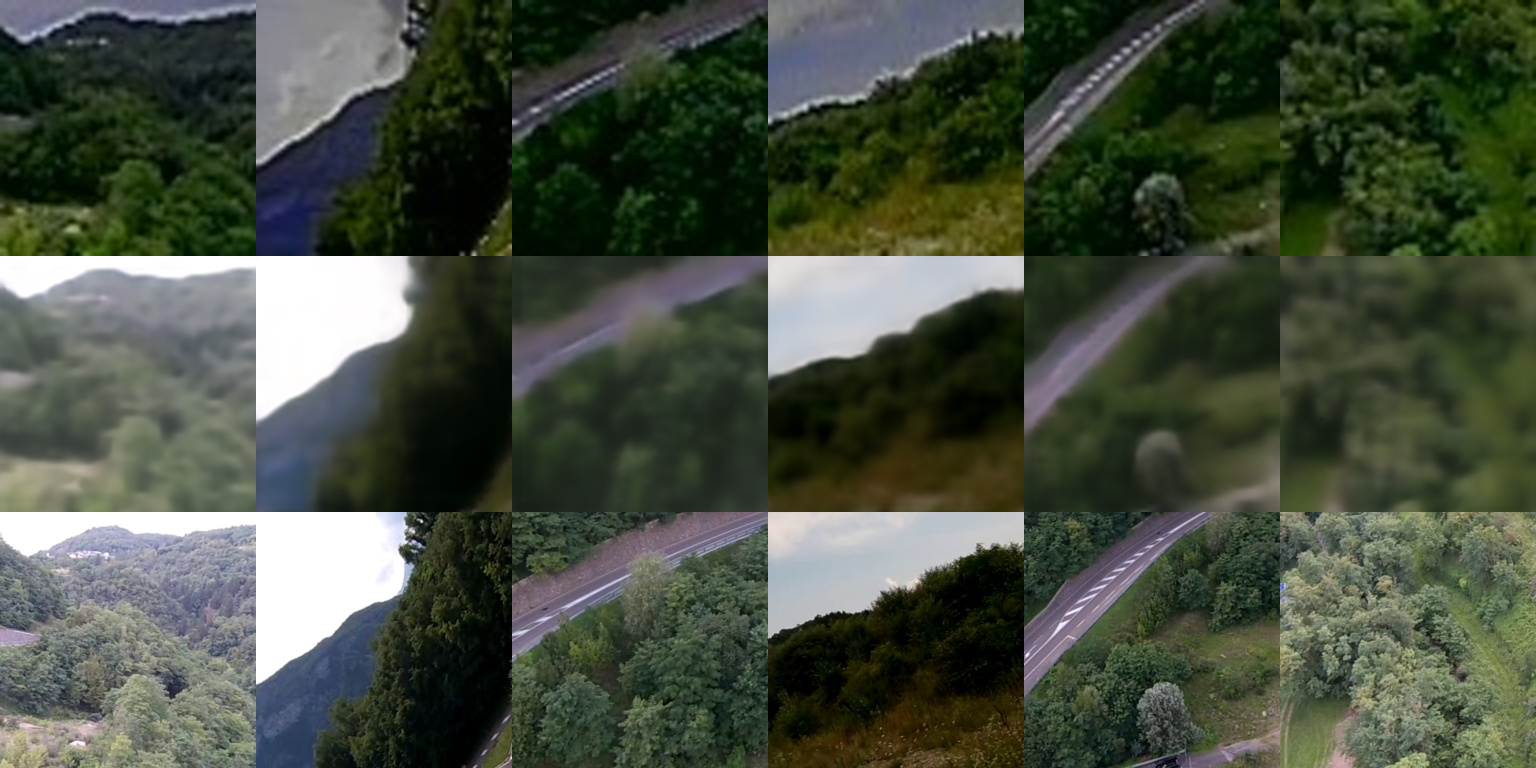
\includegraphics[width=1\textwidth]{figures/allegati/swinir_64_patches.png}
  \caption{From the 64 to 256 patches dataset.}
  \label{img:esrgan_att}
\end{figure}

\begin{figure}[H]
  \centering
  \includegraphics[width=1\textwidth]{figures/allegati/swinir_128.png}
  \caption{From the 128 to 512 dataset.}
  \label{img:esrgan_att}
\end{figure}

\subsection{HAT-L}

\begin{figure}[H]
  \centering
  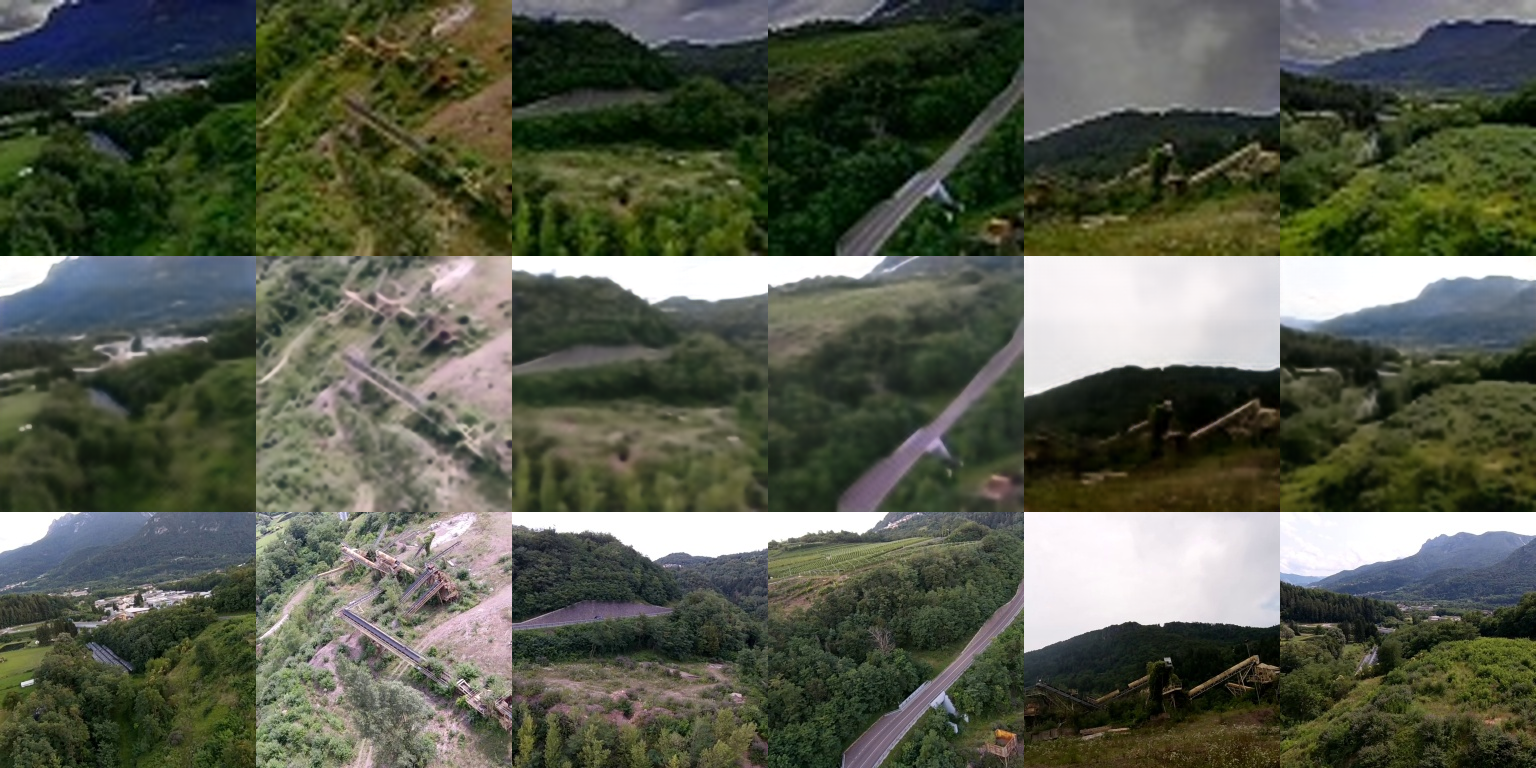
\includegraphics[width=1\textwidth]{figures/allegati/hatl_64.png}
  \caption{From the 64 to 256 dataset.}
  \label{img:esrgan_att}
\end{figure}

\begin{figure}[H]
  \centering
  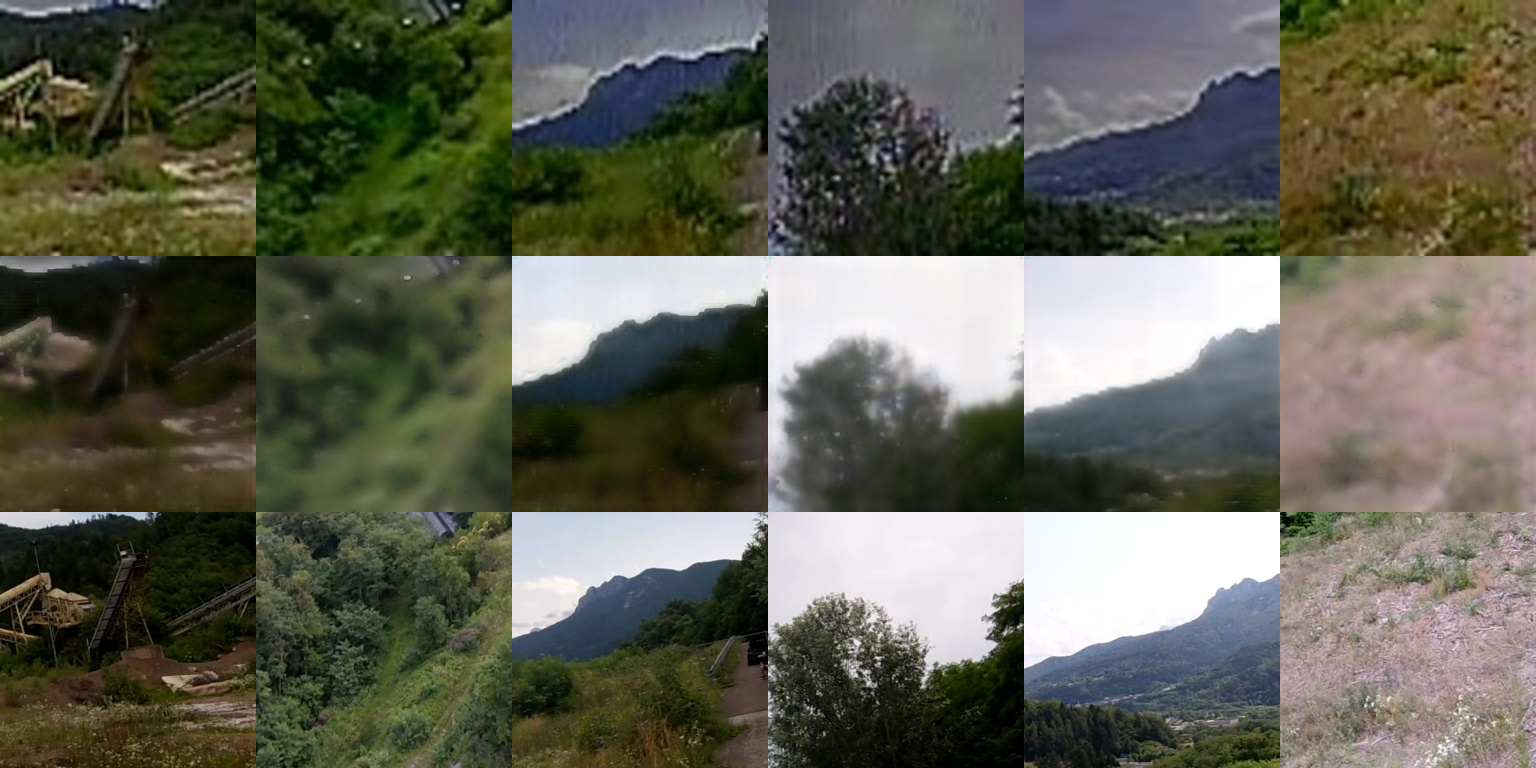
\includegraphics[width=1\textwidth]{figures/allegati/hatl_64_patches.png}
  \caption{From the 64 to 256 patches dataset.}
  \label{img:esrgan_att}
\end{figure}
